\documentclass[en]{../../../eplnotes}

\usepackage{../../../eplunits}
\usepackage{bbm}

\DeclareMathOperator{\BC}{BC}
\DeclareMathOperator{\SR}{SR}
\DeclareMathOperator{\PS}{PS}
\DeclareMathOperator{\DES}{DES}
\DeclareMathOperator{\LB}{LB}
\DeclareMathOperator{\LCB}{LB}
\DeclareMathOperator{\ELB}{ELB}
\DeclareMathOperator{\ALH}{ALH}
\DeclareMathOperator{\DP}{DP}
\DeclareMathOperator{\EDP}{EDP}
\DeclareMathOperator{\MC}{MC}

\DeclareMathOperator{\E}{\mathbb{E}}

\newcommand{\Tph}{T_\mathrm{ph}}
\newcommand{\Top}{T_\mathrm{op}}
\newcommand{\fop}{f_\mathrm{op}}

\renewcommand{\a}{\mathbf{a}}
\renewcommand{\b}{\mathbf{b}}
\newcommand{\xor}{\oplus}

\usepackage{qtree}

\hypertitle{Secure Electronic Circuits and Systems}{8}{ELEC}{2760}
{Benoît Legat}
{François-Xavier Standaert}

\paragraph{Discussion link}
\url{http://www.forum-epl.be/viewtopic.php?t=13109}

\section{Introduction}
\paragraph{Discussion link}
\url{http://www.forum-epl.be/viewtopic.php?t=12055}
\subsection{Perfect Secrecy}
Suppose we want perfect secrecy.
\[ \Pr[C = c \mid P = p_0] = \Pr[C = c \mid P = p_1]. \]
The attacker gain absolutely no information on $P$ when watching $C$
because they are independent so whatever is its computational power or its time,
trying to find $P$ is hopeless.

It can be proven that the key must be as long as the message.

With a key as long as the message it can be done with the One Time Pad (OTP).
The same key cannot the used twice because if we get
$c = p \oplus k$ and $c' = p' \oplus k$, we have $c \oplus c' = p \oplus p'$
so we do not have any secrecy.
Of course if we use $k$ twice it is like using a key 2 times shorter than the message so we know that we cannot have perfect secrecy.

Have such long key is problematic,
there is also the problem of sharing those key,
if Alice and Bob achieve to share this key as long as the message privately,
why don't they share the message directly.

\subsection{Conditional security}
We come to the conditional security.
We rather want that if the adversary has limited computational power (need to be polynomial time),
we cannot break the scheme with probability that is not exponentially low.
\begin{figure}[!ht]
  \centering
  \begin{tikzpicture}[x=1cm,y=.05cm]
    \draw[domain=0:6] plot
    (\x, {2^(\x)-1});
    \draw[domain=0:6] plot
    (\x, {(\x)^2});
    \node[right] at (6,36) {encryption/decryption};
    \node[right] at (6,63) {breaking};
    \draw[thick,->] (0,0) to (0,65);
    \node[left] at (0,65) {complexity};
    \draw[thick,->] (0,0) to (7,0);
    \node[below] at (7,0) {security parameter};
  \end{tikzpicture}
  \caption{We want breaking to be a lot slower than encryption/decryption for large security parameter.
  Typically this is the case if breaking is exponential and encryption/decryption is polynomial.}
\end{figure}

\subsection{Formal security definition}
How can we define security formally ?
Can we say that recovering the key is hard ? No because a scheme that do not use the key is insecure but it is impossible to find the key.

We define a Pseudo Random Generator (PRP) as an encryption scheme such that if an efficient adversary choose $q$ plaintext of $n$-bit and then receives either the $q$ encryptions or the $q$ values under a real permutation (the same for the $q$ plaintext), and try to guess whether it is random strings or not.
Its probability of success ${} - 1/2$, i.e. its \emph{advantage}, is negligible in $n$.

Note that we need to assume that the adversary is efficient (e.g. $\ll 2^n$) and only ask for a negligible probability because
it an unbounded adversary can disinguish a PRP from a real permutation (a permutation is a bijective function).
Indeed there are $(2^n)!$ different permutation and since the PRP is only parametriced by an $n$-bit key,
there are only $2^n$ different permutation that the PRP can be, it is a exponentially smaller than $(2^n)!$.

For an encryption scheme is CPA (Chosen Plaintext Attack) secure if when we always give the efficient adversary the $q$ encryptions
and then allow it to choose two new plaintexts (using the new information available) for which we either reply either the encryption of the first or the second, then the advantage is negligible in $n$.

We can see that to be CPA secure the scheme \emph{must be probabilitic}.
Otherwise the adversary can just take the two new plaintexts in the $q$ for which we know the encryption
and he will win everytime.
Note that an encryption is always an injective function for the decryption to work so we know that the encryptions are different.

Luckily it is easy to build CPA secure scheme from PRP using techniques such as CBC.

\section{Block Ciphers}
\paragraph{Discussion link}
\url{http://www.forum-epl.be/viewtopic.php?t=11822}
\subsection{Warm up questions}
There are $(2^n)!$ permutations so the probability that a permutation $P$ picked uniformly at random in the set of all permutations is a given permutation is $\frac{1}{(2^n)!}$.
For 2 $n$-bits strings, $x, y$ chosen unformly at random, we have
\[ \Pr[Y = y] = \Pr[P(x) = y] = \frac{1}{2^n} \]
because (we define $\mathbbm{1}_{Q}$ which is $1$ if $Q$ is true and $0$ otherwise)
\begin{align*}
  \Pr[P(x) = y]
  & = \sum_p \Pr[P = p] \mathbbm{1}_{p(x) = y}\\
  & = \sum_p \frac{1}{(2^n)!} \mathbbm{1}_{p(x) = y}\\
  & = \frac{1}{(2^n)!} \sum_m  \mathbbm{1}_{p(x) = y}\\
  & = \frac{(2^n-1)!}{(2^n)!}\\
  & = \frac{1}{2^n}.
\end{align*}
We have $(2^n-1)!$ permutation $p$ such that $p(x) = y$ because the output of $x$ is fixed,
the ouptut of the next $x$ can be chosen in all the $b$-bits strings but $y$ so $2^n-1$ choice,
the next one has $2^n-2$ choices, ...

Consider now a block cipher $\BC \colon \{0,1\}^n \times \{0,1\}^n \to \{0,1\}^n : y = \BC_k(x)$.
As we have seen for the decryption to be unique, for a fixed $k$ it should be injective.
Since for a fixed $k$ there are as many $x$ than $y$ and it is injective, it must be surjective too.

There are only $2^n$ such bijection (one for each key), it is a lot smaller than the number of permutation: $(2^n)!$.
For a fixed $x$, it is not necessarily a bijection (but it is better if it is).

\subsection{How to construct PRPs?}
We first see how to construct a $1$PRG.
Suppose the key is a prime number $p$ and a generator $g$ of $p$,
i.e. an integer such that $g^i \not\equiv 1 \pmod{p}$ for $0 < i < p-1$.
For a seed $s$, we compute $x_1 \equiv g^{s} \pmod{p}$ and output a bit 1 if $x_1 < \frac{p-1}{2}$ and 0 otherwise.

If we continue, $x_2 = \equiv f^{x_1} \pmod{p}$, output 1 if $x_2 < \frac{p-1}{2}$ and 0 otherwise,
$x_3 = \equiv f^{x_2} \pmod{p}$, ...
Then we get a $n$PRG.
Note that if the probability of success of the adversary for the $1$PRG is $\SR_1$,
since he can attack the $n$ different $1$PRG separately, its success rate for the $n$PRG with $N$ iterations is
\begin{align*}
  \SR_n
  & = 1 - (1-\SR_1)^N\\
  & \approx 1 - (1-N\SR_1)\\
  & = N\SR_1\\
  & \approx q \frac{1}{2^n}.
\end{align*}
This is problematic if $q = 2^n$.

Note that for a PRG, the adversary doesn't know the seed, he just sees the output and try to see if it looks random.
For a PRF/PRP, the adversary knows (and even choose) the input.

We can build an PRF from a $n$PRG.
We start with the seed $s$ of $n$ bits.
We generate $2n$ bits using the $n$PRG and if the first bit of the input is 0 we keep the $n$ first bits and if it it $1$ we keep the $n$ last bits.
Then we use those $n$ bits as seed for our $n$PRG and generate $2n$ bits,
if the second bit of the input is 0 we keep the $n$ first bit and otherwise the $n$ last bit,
then we use those $n$ bits as the seed for our $n$PRG and generate $2n$ bits, ...

\begin{figure}[!ht]
  \centering
  \Tree
  [.{seed $s$}
    {$x_1 = 0$\\$n$ first bits}
    [.{$x_1 = 1$\\$n$ last bits}
      [.{$x_2 = 0$\\$n$ first bits}
        [.{$x_3 = 0$\\$n$ first bits}
          {$x_4 = 0$\\$n$ first bits}
          {$x_4 = 1$\\return the $n$ last bits}
        ]
        {$x_3 = 1$\\$n$ last bits}
      ]
      {$x_2 = 1$\\$n$ last bits}
    ]
  ]
  \caption{PRG to PRF if the input is $x = 1001$.}
\end{figure}

To build a PRP from the PRF we use Luby-Rackoff.
If the advantage for the PRF is $\epsilon$,
for the PRP it won't be more than $3\epsilon + \frac{q^2}{2^{n+1}}$.
It is problematic for $q = \bigoh(2^{n/2})$ but we can't really do better because of the Birthday Paradox.

The drawback of this technique is that the time for the PRP is $3n^2$ times the time for the $1$PRG.

\subsection{Time-memory tradeoffs}
Suppose we have a PRP with keys of $k$ bits and messages of $n$ bits.

Once we have a plaintext, ciphertext pair, we can recover the key in $\bigoh(2^k)$ time complexity and $\bigoh(1)$ memory complexity.
We need no precomputation for that.

If we are allowed to choose the plaintext (CPA),
we can, for a fixed plaintext,
precompute the whole table where for each of the $2^k$ keys we compute the corresponding ciphertext.

Then for each ciphertext we can retrieve the key in $\bigoh(1)$.
The online time complexity is therefore $\bigoh(1)$ but the memory complexity and time complexity of the precomputation is $\bigoh(2^k)$.
However the precomputation is done only once.
Still this is not practical for large $k$.

We cannot reduce the time complexity of the precomputation but we can reduce the memory complexity.
Assume that for some $m$, we choose $m$ different keys $x_{i,0}$
and then for each of them we compute the encryption $y_{i,1}$ of the fixed plaintext using $x_{i,0}$ as key.
Suppose we have a reduction function $g \colon 2^n \to 2^k$.
We set $x_{i,1} = g(y_{i,1})$ note that now $x_{i,1}$ has also the size of a key.

We repeat it $t$ times for each of the $m$ keys (time complexity $\bigoh(mt)$ for the precalculation)
and only remember $x_{i,0}$ and $x_{i,t}$ for each $1 \leq i \leq m$ (space complexity $\bigoh(t)$).

For the online (CPA!) attack, we take the ciphertext, reduce it using $g$ and then encrypt/reduce with $g$ $t$ times (or less)
until we arrive at $x_{i,t}$ for some $i$.
If we do we can find the key (if we needed $j$ steps it is $x_{i,t-j}$) by starting again at $x_{i,0}$ and doing $t-j$ steps.
If after $t$ steps we have been any of the $x_{i,t}$ that means that the key is not in the table.
Is it possible even if $mt \geq 2^n$. Yes because it may happend that $x_{i,j} = x_{i',j'}$ for $i \neq i'$ or $j \neq j'$.
In such case, there are redundance in the table.

If we compute $x_{1,t}$ then $x_{2,t}$ then $x_{3,t}$, ...
We can see that when we compute $x_{i,j}$ we have generated less than $ti + j$ so the probability to get a new key not encountered yet if $x_{i,j-1}$ was new is at least $1 - \frac{ti+j}{2^n}$, let's approximate it by $1-\frac{ti}{2^n}$.
Since we also need that $x_{i,j-1}$ is new,
we can prove by induction that the probability that $x_{i,j}$ is new is at least
\[ \Big(1 - \frac{it}{2^n}\Big)^j \]
Therefore the number of keys we generate is
\[ \sum_{i=1}^m \sum_{j=1}^t \Big(1 - \frac{it}{2^n}\Big)^j. \]

For an attack to success, the key must be among them so the success probability of an attack is at least
\[ \PS_{\mathrm{tab}} \geq \frac{1}{2^k}\sum_{i=1}^m \sum_{j=1}^t \Big(1 - \frac{it}{2^n}\Big)^j. \]
It is well known that $1 - x \approx \exp(-x)$.
So the success rate is
\[ \PS_{\mathrm{tab}} \approx \frac{1}{2^k}\sum_{i=1}^m \sum_{j=1}^t \exp\Big(\frac{ijt}{2^n}\Big). \]
The last term of this sum is $\frac{mt^2}{2^n}$.
We see that it is a waste of time to take $mt^2$ larger than $2^n$.

To further increase the probability of success we can generate $r$ tables with \emph{different} $g$.
Note that since $g$ is differente if in one table we encounter the same $x_{i,j}$ than with another one it won't mean
that the following $x_{i,j'}$ for $j' > j$ will also be the same.
The probability of success will be
\[ \PS = 1 - (1 - \PS_{\mathrm{tab}})^r \]

We see that the precomputation time complexity is $\bigoh(mtr)$,
the memory complexity is $\bigoh(mr)$, and the online time complexity is $\bigoh(tr)$.

Typical values of $m,t,r$ are $m = t = r = 2^{k/3}$, which gives
a precomputation time complexity of $\bigoh(2^k)$,
a memory complexity of $\bigoh(2^{2k/3})$, and the online time complexity is $\bigoh(2^{2k/3})$.

\subsection{Attacks against 2DES}
DES is too short (56 bits).
Can we increase the number of key bits while still keeping DES (e.g. reuse existing hardware) ?
What if we define 2DES which has 112 bits key $(k_1,k_2)$ and encrypt $x$ as $\DES_{k_1}(\DES_{k_2}(x))$?
We can use a Meet in the Middle Attack !
Suppose we have a plaintext/ciphertext pair $(x,y)$.
For each of the $2^{56}$ keys $k_1$ we compute $\DES^{-1}_{k_1}(y)$ and store it in a table (memory complexity $2^{56}$).
Then for each of the $2^{56}$ keys $k_2$ we compute $\DES_{k_2}(x)$ and do a table lookup ($\bigoh(1)$).

What is used instead of 2DES is 3DES (pronounced ``Triple-DES'') which takes a key of $3 \cdot 56$ bits and encrypt $x$ as
$\DES_{k_1}(\DES_{k_2}(\DES_{k_3}(x)))$.
Not that the security is not more than $2^{112}$ because of the Meeth in the Middle Attack.

\subsection{Attack against OFB/CFB}
OFB basically generate a one-time pad so for the same reason than
with the one time pad, it cannot be used twice with the same IV.

The CFB is a one-time pad for the first ciphertext.

For CBC if $c_i$ is the same for two ciphertext the xors of the $p_i$ will equal the xor of the $c_{i-1}$.
The probability to have a collision for $i$th ciphertext is $i/2^n$ so the probability to have no collision is
\[ \prod_{i=1}^q \Big(1 - \frac{i}{2^n}\Big) \approx \prod_{i=1}^q \exp\frac{i}{2^n} = \exp\Big(\frac{1}{2^n} \sum_{i=1}^q\Big) = \exp\frac{q(q+1)}{2^{n+1}} \approx \exp \frac{q^2}{2^n}. \]
so we cannot use more than $q = 2^{n/2}$.


\subsection{Semi-Generic Attacks}
In the Luby-Rackoff of DES, the key scheduling just permutations of bits of the key.
Therefore if the key is $000\ldots0$ or $111\ldots1$, all the subkeys are the same.
Since the decryption is the same Luby-Rackoff than the decryption but with the subkeys used in the order,
the encryption of DES and the decryption are the same for those 2 keys.
Hence, encrypting twice does nothing, it is called an involution.

Let $\overline{x}$ be the string for which we inverse each bit of $x$.
We can see that $\overline{\DES_k(x)} = \DES_{\overline{k}}(\overline{x})$.
\begin{proof}
  For the PRF inside $\DES$, $F(\overline{R}_i, \overline{K}_i) = F(R_i,K_i)$.
  Therefore for an input $(L_1',R_1') = (\overline{L}_1,\overline{R}_1)$ and $K' = \overline{K}$, we have
  \begin{align*}
    (L_2',R_2')
    & = (R_1', L_1' \xor F(R_1',K_1'))\\
    & = (\overline{R_1}, \overline{L_1} \xor F(\overline{R_1},\overline{K_1}))\\
    & = (\overline{R_1}, \overline{L_1} \xor F(R_1,K_1))\\
    & = (\overline{R_1}, \overline{L_1 \xor F(R_1,K_1)})\\
    & = (\overline{L_2}, \overline{R_2}).
  \end{align*}
\end{proof}

\subsubsection{Attack on 1 round DES}
If there is only 1 round, and we know a ciphertext/plaintext pair,
we can find the input and output of the PRF $F$ of DES for the first subkey.
Since the subkey has only $48$ bits we can break it with a SR of $2^{48}$.

Now actually $F$ is not composed of one big S-box of 48 bits because it wouldn't be efficient
so we have $8$ small S-boxes of $6$ bits each.
Since we have the input and output of $F$ there has been not diffusion,
we can get the input and output of each S-box and attack it to find the part of the key xored with the input of each S-box.
SR becomes $8 \cdot 2^6$.

\subsubsection{Attack on DES with no key schedule}
If the same key was used for each round, we could use a slide attack.
Let $N_R$ be the number of rounds, $k$ be the same key used for each round and $R_k$ be one round (i.e. $\DES_k(x) = R_k^{N_R}(x)$).

Suppose we have 2 plaintext/ciphertext pairs for which the output of the ciphertext of the first one $c_0$ is the output of the $(R-1)$th round of the second one.
We know that $R_k(c_0) = c_1$.
As we have seen, breaking one round is easy to from $c_1$ and $c_0$ we find $k$.
Note that we also have that $R_k(p_0) = p_1$ so we can find $k$ this way too.

\begin{figure}[!ht]
  \centering
  \begin{tikzpicture}
    \node[left] at (0,1) {$p_0$};
    \draw (0,1) to (1,1);
    \node[left] at (1.5,1) {$R$};
    \draw (1.5,1) to (2.5,1);
    \node[right] at (2.5,1) {$\cdots$};
    \draw (3.2,1) to (4.2,1);
    \node[left] at (4.7,1) {$R$};
    \draw[->] (4.7,1) to (5.7,1);
    \node[right] at (5.7,1) {$c_0$};
    \node[left] at (1,0) {$p_1$};
    \draw (1,0) to (2,0);
    \node[left] at (2.5,0) {$R$};
    \draw (2.5,0) to (3.5,0);
    \node[right] at (3.8,0) {$\cdots$};
    \draw (4.7,0) to (5.7,0);
    \node[left] at (6.2,0) {$R$};
    \draw[->] (6.2,0) to (7.2,0);
    \node[right] at (7.2,0) {$c_1$};
  \end{tikzpicture}
  \caption{Slide Attack}
\end{figure}

Now in a more reallistic setting we just have 2 plaintext/ciphertext pairs and we don't know whether $R_k(c_0) = c_1$.
If we look for the key $\tilde{k}$ such that $R_{\tilde{k}}(c_0) = c_1$ it is not sure that $\tilde{k} = k$.
We can check whether $\DES_{\tilde{k}}(p_0) = c_0$ and if it is the case, we have good chance that $\tilde{k} = k$.
In practice we find $\tilde{k}$ such that $R_{\tilde{k}}(c_0) = c_1$ and just check that $R_{\tilde{k}}(p_0) = p_1$,
it is rather to do one round than $N_R$ rounds.

From 2 pairs, the chance of having $\tilde{k} = k$ is $1/2^n$.
However, if we have $q$ plaintext/ciphertext pairs, we have $q^2$ pairs.
That's the birthday paradox, we only need $q = 2^{n/2}$ pairs to have a collision.
We say that the \emph{data complexity} is $\bigoh(2^{n/2})$.

However it is important to note than usually, once we have a new plaintext/ciphertext pair,
we can check in $\bigoh(1)$ whether there is a collusion with table lookup.
Here however, we need, for each pair to compute $\tilde{k}$ and do the check.
Therefore the time complexity is $\bigoh(2^n)$ even if the data complexity is $\bigoh(2^{n/2})$.

Note that for DES, the only $32$ bits are used in $F$ so it is ``like if $n$ is $n/2$'' so the data complexity is $\bigoh(2^{n/4})$
and the time complexity is $\bigoh(2^{n/2})$.

\subsection{Piling-up lemma}
Let $V_1$ and $V_2$ be two independent random bit variables for which
\( \Pr[V_i = 0] = p_i. \)
We see that
\begin{align*}
  \Pr[V_1 \xor V_2 = 0]
  & = p_1p_2 + (1-p_1)(1-p_2)\\
  & = 1 + 2p_1p_2 - p_1 - p_2\\
  & = \frac{1}{2} + 2(1/4 + p_1p_2 - p_1/2 - p_2/2)\\
  & = \frac{1}{2} + 2(p_1 - 1/2)(p_2 - 1/2)\\
  & = \frac{1}{2} + 2\varepsilon_1 \varepsilon_2.
\end{align*}
where
\( \varepsilon_i = p_i - 1/2 \)
is the called the \emph{bias}.

We can generalize it by induction:
\[ \Pr[V_1 \xor \cdots \xor V_n = 0] = \frac{1}{2} + \frac{1}{2^{n-1}} \prod_{i=1}^n \varepsilon_i. \]

\subsection{Divide and Conquer attacks}
If we combine linear relations on several S-boxes and
get a linear relation involving the input bits, the output bits and a lot of key bits of each round,
we can apply linear cryptanalysis.
Let $\a$ be the mask with a $1$ if the corresponding input bit is used in the linear approximation and a 0 otherwise.
Let $\b$ be the similar mask for the output.

We define an S-box be \emph{active in the partial decryption} if $\a$ has a 1 for the the input of this S-box.
We consider the bits of the key that are xored to the input of S-box that are active in the partial decryption.
For each plaintext/ciphertext pair,
we try all the possible values for those bits and for each of them we do a partial encryption of the plaintext
for the S-boxes active in the partial decryption (now you understand why we call them like that)
and look if the linear approximation (removing the key bits in the expression) gives 0 or 1.

We define the experimental bias for as the number of plaintext/ciphertext pair which gives the same value for the linear approximation (divided by the number of p/c pairs).
We can hope that the key bits that maximize this experimental bias are the bits of the key.

To find other key bits, we consider other approximation for which the S-box active in the partial decryption are different.
This is a divide and conquer approach.

Note that we remove the bits of the key in the linear approximation because their value does not change since the key does not change
and we do not care if the value of the linear approximation is 0 or 1,
we just want it to be biased.

Not also that we can use different paths $\Omega$ for the same $\a$ and $\b$ so the keys used in the linear approximation is not unique.

\subsection{Data complexity}
Let $\epsilon$ be the bias of the linear approximation.
We see with the Piling up lemma that it depends on the bias on a single S-box and the number of active S-boxes.
It can be shown that the number of plaintext-ciphertext necessary is $1/\epsilon^2$
(note that $\epsilon$ is the euclidean distance betweent the uniform distribution and the distribution of the linear approximation).

Therefore, we can increase the data complexity by
\begin{itemize}
  \item increasing the number of rounds (we'll see about take later),
  \item increasing the number of active S-boxes,
  \item decreasing the bias of an active S-box.
\end{itemize}

And we can increase the time complexity by limitting the possible ``division''
of the divide and conquer approach, i.e.
by increasing the number of S-boxes active in the partial decryption.

\paragraph{The AES Rijndael}
The AES Rijndael is not a Feistel cipher,
it is a key alternating cipher.

We need \emph{confusion} and \emph{diffusion} to mix up plaintext and key.
Even designers of AES do not know why they did the key scheduling the way they did it.

Note that it is not Markov since key schedule does not produce independent subkeys.

\subsection{The wide-trail strategy}
Let us see now if a wide-trail of rounds is a good idea to decrease $\epsilon$.
If we double the number of round, we double the number of active S-boxes so $\epsilon$ is squared, no ?
That is not so simple.
The limitation are:
\begin{itemize}
  \item We assume that the subkeys are independent;
  \item We assume that each key is equivalent: $LB(\a,\b,\hat{k}) \approx ELB(\a,\b)$;
  \item It is correct to say that $\lim_{N_R \to \infty} \LCB(\Omega) = 0$,
  \item but \emph{not} to say that $\lim_{N_R \to \infty} \LB(\a,\b) = 0$.
\end{itemize}

% If we iterate 2 8-bit Sbox, we won't get 2^{-6}, only 2^{-3}.
% The iteration is to have like a 128-bit S-box

Why doesn't $\LB(\a,\b)$ tend to 0 ?
In fact, there are not only one path $\Omega$ from $\a$ to $\b$.
It is not at all obvious to see it,
but a good model to explain why $\LB(\a,\b)$ does not tend to zero is the following.
Let $\ALH(\a,\b)$ be the set of all paths.
Each path has different subkey bits appearing in their linear approximation (but we don't care about that here).

For some key $K$, a path could be biased and other paths not.
However, if one path is biased, we will see a bias for $\a$ and $\b$ for that key
(interestingly, seen from $\a$ and $\b$ other paths will be biased too even though they are not biased along the path).
The probability to be biased is therefore more like the probability that it is biased for at leas one of the path which is
upper bounded by the sum of the probabilities
\[ \LB(\a,\b;K) = \sum_{\Sigma \in \ALH(\a,\b)} \LCB(\Omega,\tilde{K}). \]
If we increase the number of round,
$\LCB$ decreases for each $\Omega$ but the number of path increases too
in such a way that $\LB$ remains constant past a certain number of rounds.

\subsection{Differential vs. characteristics}
% EDP(a,b)
% = sum_p PR[p] Pr_X[p(x xor a) = p(x) xor b]
% = sum_p Pr[p] sum_x Pr[x] 1_(p(x xor a) = p(x) xor b)
% = 1/(2^n)! sum_x sum_x Pr[x] 1_(p(x xor a) = p(x) xor b)
% = 1/(2^n)! sum_p 1_(p(x xor a) = p(x) xor b)
%            --------------------------------
%            = perms: x -> alpha
%                     x xor a -> alpha xor b
% -> 1/(2^n)! (2^n)!/(2^n-1) = 1/(2^n-1)

\begin{align*}
  \EDP(\a,\b)
  & = \sum_p \Pr[p] \Pr_x[p(x \xor a) = p(x) \xor b]\\
  & = \sum_p \Pr[p] \sum_x \mathbf{1}_{p(x \xor a) = p(x) \xor b} \Pr[x]\\
  & = \frac{1}{(2^n)!} \sum_x \Pr[x] \sum_p \mathbf{1}_{p(x \xor a) = p(x) \xor b}\\
  & = \frac{1}{(2^n)!} \sum_x \Pr[x] 2^n(2^n-2)\\
  & = \frac{1}{(2^n)!} 2^n(2^n-2)\\
  & = \frac{1}{2^n-1}.
\end{align*}
Note that we have $2^n(2^n-2)$ because we have $2^n$ choices for $p(x)$ but once we have chosen it
we have no choice for $p(x \xor a)$ then we have $2^n-2$ choices left for the other inputs.

Differential cryptanalysis is more useful in the case of related keys,
e.g. encrypt everything with $k_1$, $k_2$ then $k_1 \xor k_2$.
AES has troubles with related keys.

% Group: <G, +>
% -> closed
% -> associative
% -> neutral
% -> inverse
% -> (commulative)
%
% Field: <F, +, x>
% - <F,+> additive group with neutral 0
% - <F\0, x> multiplicative group with neutral 1
%
% Crypto => finite fields
% Theorem: FF of order m <=> m = p^n (where p is prime)
%
% Extension fields (for efficiency)
% a(x) = a_7 x^7 + a_6 x^6 + ... + a_1 x + a_0
% -> polynomial with a_i in F(2)
%
% Addition: a(x) + b(x)
% Mult: a(x) + b(x) mod (n(x)
% with n(x) = irreducible polynomial.
%
MixColumns is linear because it is multiplications by constants.
From a columns $a_0, a_1,a_2,a_3$, we get
\begin{align*}
  & (03 x^3 +  01 x^2 +  01 x +  02) (a_3 x^3 + a_2 x^2 + a_1 x + a_0)\\
  & =         3a_3 x^6 + 3a_2 x^5 + 3a_1 x^4 + 3a_0 x^3
            + 1a_3 x^5 + 1a_2 x^4 + 1a_1 x^3 + 1a_0 x^2\\
  & \quad {}+ 1a_3 x^4 + 1a_2 x^3 + 1a_1 x^2 + 1a_0 x
            + 2a_3 x^3 + 2a_2 x^2 + 2a_1 x   + 2a_0\\
  & =         3a_3 x^2 + 3a_2 x^1 + 3a_1     + 3a_0 x^3
            + 1a_3 x^1 + 1a_2     + 1a_1 x^3 + 1a_0 x^2\\
  & \quad {}+ 1a_3     + 1a_2 x^3 + 1a_1 x^2 + 1a_0 x
            + 2a_3 x^3 + 2a_2 x^2 + 2a_1 x   + 2a_0\\
  & = (3a_0 + 1 a_1 + 1 a_2 + 2a_3)x^3 + (1a_0 + 1a_1 + 2a_2 + 3a_3)x^2\\
  & \quad {} + (1a_0 + 2a_1 + 3a_2 + 1a_3)x + (2a_0 + 3a_1 + 1 a_2 + 1 a_3).
\end{align*}

The only non-linearity is the S-boxes so we try to make the most of them active.
%
% There is analysis for 4bit S-boxes ((2^4)! is small)
% Not for 8bits S-boxes ((2^8)! is huge)
%
% We are not in the field of provable security.
%
% At the moment, nobody really knows how to do the key scheduling.
% There are related key attacks.
%   _   _
% _| |_| |_...
%
% _|\_|\


\section{Hardware Implementations}
\paragraph{Discussion link}
\url{http://www.forum-epl.be/viewtopic.php?t=11843}

In 1 cycle, 3 things happens,
we read in memory, do the operation and write in memory.
The critical path $\Tph$ is only the time of the operation,
the operation delay $\Top$ is the time of the full cycle
and the operation frequency $\fop = 1/\Top$.

\subsection{Design tradoffs}
Si on considère un pipeline (interne au round AES) idéal, le débit (throughput) est multiplié par 2:

For implementation 1 (without pipelining),
the latency (the number of cycle needed for 1 plaintext) is \SI{11}{cycles} (1 cycle per round)
so the throughput is
\[ \frac{\SI{128}{bits}}{\SI{11}{cycles} \cdot \Top} \]
For implementation 2 (with pipelining),
the latency is now \SI{22}{cycles} because there is 2 cycles per round.
The operation dealy $\Top$ however is twice smaller
so the throughput is
\[ \frac{2 \cdot \SI{128}{bits}}{\SI{22}{cycles} \cdot \Top/2} \]
We produce $2 \cdot \SI{128}{bits}$ because we can produce
2 ciphertexts at the same time since we have added a memory.
We see that the thoughput has doubled.
In practice however the operation delay for the implementation 2 is bigger than $\Top/2$.

Pipelining cannot always be done,
it can be done forECB
but not for CBC because it needs the result of the previous one for the next one.

To do 2 ciphertext at the same time, we can also have 2 implementation of a round with a memory after the first one and a memory after the second one. This won't change $\Top$ nor the latency but the throughput will be doubled.

To double the throughput we can also have 2 parallel implementation of an AES round but that is less efficent since it costs 2 multiplexor.

\subsection{Application to block ciphers}
Consider the logic blocks LB1 (\figuref{LB1}) and LB2 (\figuref{LB2}) for FPGA.
\begin{figure}[!ht]
  \centering
  \begin{subfigure}[b]{0.45\textwidth}
    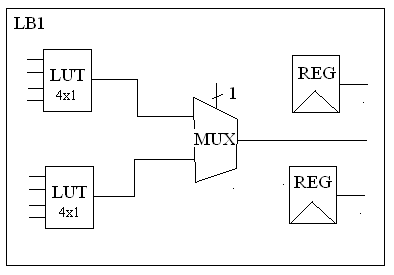
\includegraphics[width=\textwidth]{LB1.png}
    \caption{LB1}
    \label{fig:LB1}
  \end{subfigure}
  \begin{subfigure}[b]{0.45\textwidth}
    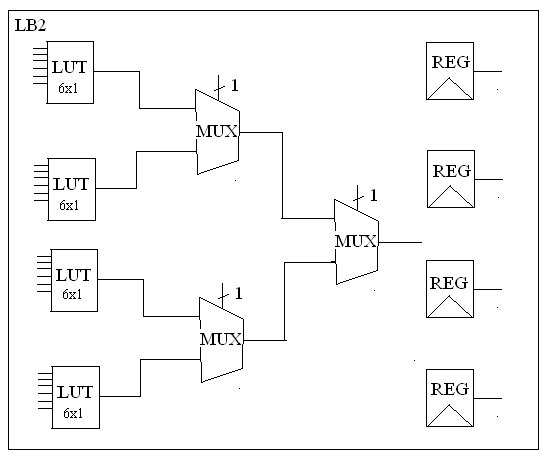
\includegraphics[width=\textwidth]{LB2.png}
    \caption{LB2}
    \label{fig:LB2}
  \end{subfigure}
  \caption{Different logic blocks for FPGA}
\end{figure}
\begin{figure}[!ht]
  \centering
  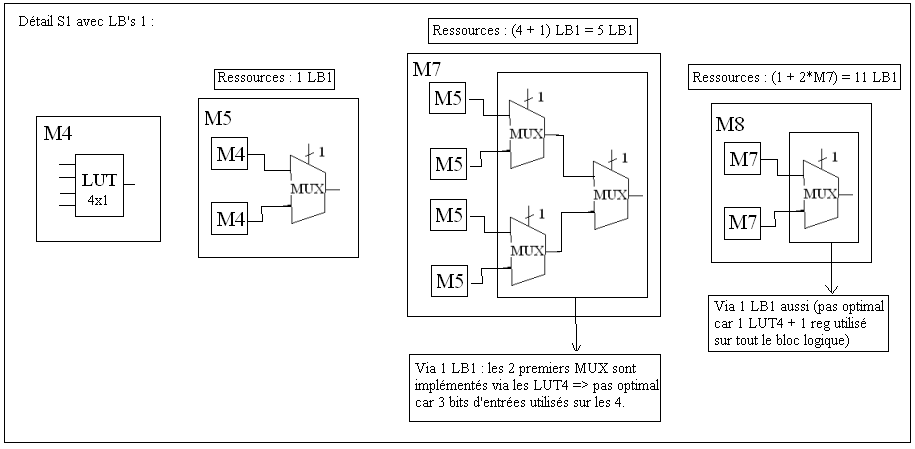
\includegraphics[width=\textwidth]{S1LB1.png}
  \caption{Implementation of $S_1$ in LB1.}
  \label{fig:S1LB1}
\end{figure}

\subsubsection{S-box implementations}
Suppose we want to implement $S_1$ and $S_2$ (see slides).
The minimum memory cost for $S_1$ is $2^8 \cdot 8 = 2048$ bits because we need the output for the $2^8$ inputs and the output
are $8$-bits.
For $S_2$ we have 6 $4$-bit S-boxes so the minimum memory cost is $(2^4 \cdot 4) \cdot 6 = 384$ bits.

\begin{description}
  \item[$S_1$ in LB2]
    To implement $S_1$ in LB2, we use 1 LB2 for each of the 8 output bits so we need $8$ LB2.
    Let $x_1x_2\ldots x_8$ be the input,
    we give $x_1x_2\ldots x_6$ as input for the 4 LUTs.
    For the $i$th LB2 (which needs to output the $i$th bit),
    the first LUT output the $i$th bit of the S-box for the input
    $x_1x_2\ldots x_600$,
    the second LUT for $x_1x_2\ldots x_610$
    the third LUT for $x_1x_2\ldots x_601$
    the fourth LUT for $x_1x_2\ldots x_611$.

    The two first multiplexors on the left are inputted $x_7$ and the last one is inputted $x_8$
    so that they can they the output bit of the right LUT.
    Only 1 of the four memory are used.
  \item[$S_1$ in LB1]
    The implementation of $S_1$ in LB2 is given by the \figuref{S1LB1}.
    For each bit, we need 11 LB1 so we need 88 LB1.
    For the $i$th bit,
    we have 8 LB1 used as M5,
    e.g. the 6th LB1 ouptuts the $i$th bit of
    $x_1x_2x_3x_4x_5101$.
    Then 2 LB1 are used as M7.
    The first outputs the $i$th output bit of $x_1x_2x_3x_4x_5x_6x_70$
    and the second the $ith$ output bit of $x_1x_2x_3x_4x_5x_6x_71$.

    A last LB1 is used as M8.
    To combine the 2 outputs of the M7 with $x_8$ it uses a LUT.
    Not that it would be faster to use the multiplexor but
    to skip the LUT, there should be 4 wires at the input of the multiplexor (2 from the LUT and 2 that skips the LUT).
  \item[$S_2$ in LB1]
    We need 12 LB1.
    Using 2 LB1 we can do Sa (same for the other).
    We do not use the multiplexor, each of the four LUT computes 1 bit and put it in one of the four the register.
  \item[$S_2$ in LB1]
    We can do it with 6 LB2, one for Sa, one for Sb, ...
    But also 8 LB2 (see the discussion link).
\end{description}

We need to choose whether put $S_1$ in memory,
otherwise it costs $88$ LB1's and
full 8 bits memory costs 2048 bits while
$S_2$ only costs 12 LB1's and 2048 bits.

\subsection{Block cipher design}
Consider an AES-like cipher
to be implemented in FPGA 1 with S-box $S_2$,
with MixColumn in 256 LUTs and logic depth 2 LUTs
and the full cipher iterating 11 rounds.

What is the cost of one round in LUTs?
\begin{itemize}
  \item Add Round Key : 64 LB1 (i.e. 128 LUT and 128 registers)
  \item SubByte : for one S-box, 12 LB1. There are 16 S-boxes so
    $16 \cdot 12 = 192$ LB1 (i.e. 384 LUT and 384 registers).
  \item MixColumns : 128 LB1 (i.e. 256 LUT and 256 registers).
  \item SR : 0 LUT just wire crossing.
\end{itemize}
TOTAL: 384 LB1 (i.e. 768 LUTs).

If the time for one LTU $\SI{60}{\milli\second}$, since one round has LUT in the critical path (6 stages, 1 in ARK, 3 in SubBytes (see $S_2$), 2 in MixColumns),
$\fop = 1/\SI{60}{\nano\second} = \SI{16.6}{\mega\hertz}$.

With no pipeline, the latency is 11 cycles since AES has 11 rounds
but there is only 128 registers.
If , the throughput is
\[ \frac{128}{11} \cdot \num{16.6e6} \]

With max pipeline (6 stages, 1 in ARK, 3 in SubBytes (see $S_2$), 2 in MixColumns),
there are 768 registers and the latency is 66 cycles.
Now $\fop = 6 \cdot \SI{16.6}{\mega\hertz} = \SI{100}{\mega\hertz}$ so
the throughput is
\[ 6\frac{128}{66} \cdot \num{100} \]
since there is 6 encryption in parallel.

It is however not realistic since even if
wires costs almost nothing in LUT, it is not negligeable in time.
So in practice $\fop$ is not multiplied by 6.

\begin{table}[!ht]
  \centering
  \begin{tabular}{lcccc}
                             & Area       & Latency    & Frequency & Throughput\\
    2 Round without pipeline & $\times 2$ & ${} / 2$   & ${} / 2$  & $\approx$\\
    2 Round with pipeline    & $\times 2$ & $\approx$  & $\approx$ & $\times 2$\\
    32 bit                   & ${} / 2$   & $\times 4$ & $\approx$ & $/ 4$\\
  \end{tabular}
  \caption{Comparison with 1 Round without pipeline.}
\end{table}

\section{Software Implementations}
\paragraph{Discussion link}
\url{http://www.forum-epl.be/viewtopic.php?t=11887}
\subsection{Power and energy}
Do larger device consume less or more energy/power?

Suppose we have two device with $\fop = \SI{1}{\mega\hertz}$
and $V_{\mathrm{dd}} = \SI{2}{\volt}$.
Suppose that for 8-bit, $P = I_{\mathrm{avg}} = \SI{3}{\milli\ampere}$.

We get a power of $\SI{2}{\volt} \times \SI{3}{\milli\ampere} = \SI{6}{\milli\watt}$.
so
\[ E_{\mathrm{cycle}} = \frac{\SI{6}{\milli\watt}}{\SI{1}{\mega\hertz}} = \SI{6}{\nano\joule}. \]

For a 32-bit device, $I_{\mathrm{avg}} = \SI{12}{\milli\ampere}$ so
the power is $P = \SI{2}{\volt} \times \SI{3}{\milli\ampere} = \SI{6}{\milli\watt}$ and
\[ E_{\mathrm{cycle}} = \frac{\SI{24}{\milli\watt}}{\SI{1}{\mega\hertz}} = \SI{24}{\nano\joule}. \]

\subsection{AES S-box}

\paragraph{Does it make sense to move the S-box in RAM ?}

The load instruction takes 2 cycles for the RAM and 3 for the ROM.
But it is initially in the ROM so for the RAM we must first load it from the ROM to the RAM.
The size of the S-boxes is $256$ bytes so to load it to the RAM we need $256 \cdot (3+2) = 1280$ cycles ($3$ to read the ROM, $2$ to write the RAM).
For an encryption, there are 16 S-boxes per round and 10 rounds so 160 encryptions in total.
Let $N_e$ be the number of encryptions,
with the RAM it takes $1280 + 2 \cdot 160 \cdot N_e$ and with the ROM it takes $3 \cdot 160 \cdot N_e$ so it is interesting to do the transfer to the RAM is there is more than 8 encryptions in a row.

However the implementations on microcontrolers are essentially useful for authentication which rarely requries more than one encryption in arow so the ROM is better for this case.


\paragraph{For which $n$ does the bitslice become interesting ?}
Where $n$ is the bus size.

With BitSlicing, there are \SI{17}{cycles\per bit} so
$\frac{17 \cdot 8}{n}$ cycles per S-box.

With the LUT's, there is 5 cycles per S-box.

BitSlicing is interesting if
\( \frac{17 \cdot 8}{n} < 5 \)
so for \( n > 27.2 \).

We see that BitSlicing is interesting from a bus size of \SI{32}{bits}.

\section{Side-Channel Attacks}
\paragraph{Discussion link}
\url{www.forum-epl.be/viewtopic.php?t=12017},
\url{http://www.forum-epl.be/viewtopic.php?t=12119}

\subsection{Exemplary attack against DES}
Kocher's DPA is a divide and conquer attack.
Increasing the number of rounds doesn't help since it targets the first round.
For perfect security against DPA, the power should be independent with the key.

In Kocher's DPA, we model the noise simply by the value of one bit
and the statistical test is a difference of mean.

To recover the whole keys we do the same attack on other bits (divide and conquer).

We only focus on 1 bit considering the others as noise.
In general it is better to use the 4 bits us have a better SNR.
With parallel computation it is harder to attack
because there is more noise.

There are several peak because the S-box is not perfect
so if we have good correlation at the input, it's the same at the output.
The higher peak is the correct candidate,
other hight peaks are other values with very close hamming weight.

\subsection{Improved attacks}
To improve the attack we can:
\begin{itemize}
  \item Improve the measurement setup;
  \item Do an adaptative selection of the inputs;
  \item Do a preprocessing of the traces;
  \item Improve leakage model with profiling, characterization;
  \item Exploit multiple samples, multivariate statistics (e.g. choose $y$ and $z$);
    \begin{itemize}
      \item Higher order attacks;
      \item Template attacks;
    \end{itemize}
  \item Do different statistical tests:
    \begin{itemize}
      \item Difference of mean;
      \item Correlation analyser;
      \item Bayesian classification.
    \end{itemize}
  \item Try to remove the noise, filtering;
  \item Improve the model (Hamming weight) with Proviling, Supervised Machine Learning.
\end{itemize}

For Template Attacks we can use probability and the correct key tends to 1.
Note that for the CPA with Pearson's correlation coefficient we can also have probability with confidence intervals.

\subsection{Countermeasures}
\begin{itemize}
  \item Use a huge table so there is no computation so no dependence on hamming weigth;
  \item Huge variance so we need much more samples (SNR).
    Signal is variance over the mean
    and noise is mean of the variance.
  \item Encoding the data so that they have the same hamming weigth.
\end{itemize}
Note the following about countermeasures
\begin{itemize}
  \item They are never perfect (they only make the attack harder);
  \item They can be implemented at different abstraction levels
    \begin{itemize}
      \item Physical (noise addition),
      \item Technological,
      \item HW/SW design (time/data randomization),
      \item Algorithmic/protocol (key updates).
    \end{itemize}
  \item To balance with implementation cost.
\end{itemize}
Masking and dual-rails are two typical examples of countermeasures.

\subsection{Key independence}
Under the assumption that:
\begin{itemize}
  \item Plaintext are uniformly distributed,
  \item $L_t(x_i,k) = f(x_i \xor k) \neq f(x_i;k)$,
\end{itemize}

\subsection{Asymptotic equivalences}
Under the additional assumption that:
\begin{itemize}
  \item $L_t(x_i,k) = \delta(x_i,k) + n$;
  \item $n \sim \mathcal{N}(\mu,\sigma^2)$,
    identical for all $t$
    and independent of manipulated data;
  \item The same models are used by all dinstinguishers.
\end{itemize}

Supose we normalize the leakage, i.e. $\E[L] = 0$ and $\sigma_L = 1$.
For the Pearson's Correlation coefficient, we have
\begin{align*}
  \tilde{k}
  & = \argmax_{k^*} \frac{\E[(L - \E[L])(M^{k^*} - \E[M^{k^*}])]}{\sigma_L\sigma_{M^{k^*}}}\\
  & = \argmax_{k^*} \frac{\E[LM^{k^*} - \E[L\E[M^{k^*}]] - \E[\E[L]M^{k^*}] + \E[L]\E[M^{k^*}]}{\sigma_L\sigma_{M^{k^*}}}\\
  & = \argmax_{k^*} \frac{\E[LM^{k^*} - \E[L]\E[M^{k^*}] - \E[L]\E[M^{k^*}] + \E[L]\E[M^{k^*}]}{\sigma_L\sigma_{M^{k^*}}}\\
  & = \argmax_{k^*} \frac{\E[LM^{k^*}] - \E[L]\E[M^{k^*}]}{\sigma_L\sigma_{M^{k^*}}}\\
  & = \argmax_{k^*} \frac{\E[LM^{k^*}]}{\sigma_{M^{k^*}}}\\
  & = \argmax_{k^*} \frac{\E[LM^{k^*}]}{\sqrt{\E[(M^{k^*})^2] - \E[M^{k^*}]^2}}.
\end{align*}
and for the template attack:
\begin{align*}
  \bar{k}  & = \argmax_{k^*} \prod_{i=1}^q \frac{1}{2\pi\sqrt{\sigma_L}} \exp\Big(-\frac{1}{2}\Big(\frac{l-m_i^{k^*}}{\sigma_L}\Big)^2\Big)\\
           & = \argmin_{k^*} \sum_{i=1}^q \Big(\frac{l-m_i^{k^*}}{\sigma_L}\Big)^2\\
           & = \argmin_{k^*} \sum_{i=1}^q l_i^2 - 2l_im_i^{k^*} + (m_i^{k^*})^2\\
           & = \argmin_{k^*} \E[L^2] - 2\E[LM^{k^*}] + \E[M^{k^*}]^2\\
           & = \argmax_{k^*} 2\E[LM^{k^*}] - \E[M^{k^*}]^2\\
           & = \argmax_{k^*} 2\frac{\E[LM^{k^*}]}{\E[M^{k^*}]^2} - 1\\
           & = \argmax_{k^*} \frac{\E[LM^{k^*}]}{\E[M^{k^*}]^2}.
\end{align*}

Asymptotically, $\E[M^{k^*}]$ and $\sigma(M^{k^*})$ are independent of $k^*$.
In the simple case of univariate model, they are asymptotically equivalent.

The model is more important that the comparison.

\section{Fault Attacks}
\paragraph{Discussion link}
\url{http://www.forum-epl.be/viewtopic.php?t=12120}

\subsection{How to introduce a fault}
There are different ways to introduce a fault:
\begin{itemize}
  \item Reduce supply voltage;
  \item Increase clock frequency;
  \item Glitch (IO, clock supply) (useful because localized in time, we see the error propagate);
  \item Increase temperature.
\end{itemize}

Note that with Glitch we can do it at a certain time
but with laser we can do it with a certain time \emph{and} at a certain coordinate.

Focused Ion Beam (FIB)
can cut the circuit layer by layer.
Reverse engineers often have access to it.

What is efficient agains fault attacks is rekeying when a fault is detected.

\subsection{Generic fault attacks}
If we can change each bit of the key separately,
we can set all the bits of the key to 0 except one.
Then we look at the ciphertext/plaintext pair
and check with 2 encryption what is the value of the bit we have left unchanged.
It is divide and conquer,
once we have found it we do the same for the other bits.

It is the most precise fault.
Its drawbacks are that
\begin{itemize}
  \item for an $n$-bit key, we need $n$ faults;
  \item It is a very precise fault.
    We a glitch, we can easily toggle a bit
    but setting a bit to 0 is not easy.
\end{itemize}

\subsection{Attacks against the AES}
If we change the ciphertext, we learn nothing of course.

If we introduce an error before ARK of the last round,
\begin{itemize}
  \item with a random byte error we learn nothing,
    it is like a one-time pad;
  \item with a bit toggle it is like toggling it after xoring the plaintext so we learn nothing;
  \item if we can set bits, we can simply set all bits to 0 and the ciphertext will be the last subkey.
\end{itemize}

Introduction an error before ShiftRows, is the same than before ARK since ShiftRows is just routing.

If we introduce an error before SubBytes, if it is a random byte error the output of SubByte will be a random byte
so it will be like a random byte error before ShiftRows, we learn nothing.
If we introduce an error of only one bit, we know in which byte it is but we do not know which bit,
we can find a byte of the subkey with 2 Ciphertext pairs in error and one Ciphertext without error (same Plaintext).
For each pair, we look at the output byte of the SubByte for which the input byte has a bit in error,
trace the bits after the ShiftRows and find which 8 bits of the key are xored with those 8 bits output of the SubByte.
For each values of those 8 bits (256 possibilities), we xor them with the ciphertext, undo the ShiftRows and SubByte.
We do that both with the Ciphertext in error and for the Ciphertext without error and check if the different between the input
of SubBytes is only one bit. There are exactly 8 values of the 8-bits of the key such that it is the case.

We do that for the other Ciphertext in error, we have again 8 values of the 8-bits of the key that works.
Normally (if we are not very unlucky), only one key is appears in both, we have found 8-bits of the first key !
We can do that for the 16 others bytes of the subkey.
We need $16 \cdot 2 = 32$ faulty ciphertexts.

Introducing an error before the ARK of the round 9 is the same than before SubByte of round 10.

Suppose we do a random byte fault on one byte before MixColumn of round 9.
Let $\delta$ be the random byte fault that is xored.
The column for which appear the fault is $(a,b,c,d)$.
Note that since MixColumn is linear,
\[ \MC(a \xor \delta,b,c,d) = \MC(a,b,c,d) \xor \MC(\delta,0,0,0). \]

Suppose we do not know in which of the four byte of the column it is.
There is $255 \times 4 = 1020$ possible patterns:
$(\delta,0,0,0), (0,\delta,0,0), (0,0,\delta,0), (0,0,0,\delta)$.
It affects 32 bytes at the output so we need to try $2^{32}$ keys.

The time complexity has increased from $2^8 \cdot 16$ to $2^{32} \cdot 4$
but now we only need $2 \cdot 4$ faulty ciphertext instead of $2 \cdot 16$.

Also the probability that 2 keys works for both ciphertext is smaller since
$1020/2^{32} < 8/2^8$.

If we do the random byte error before ShiftRows of round 9, SubBytes of round 9 or ARK of round 8 it does not change anything
it it still a random byte error on a single byte before MixColumns of round 9.

If the fault is before MixColumns of round 8, ShiftRows of round 8,
SubBytes of round 8 or ARK of round 7, the situation is even better,
the time complexity is still $2^{32}$ but we now only need 2 faulty ciphertexts.
This is explained by the \figuref{fault}.

\begin{figure}[!ht]
  \centering
  \begin{subfigure}[b]{0.3\textwidth}
    \begin{tikzpicture}
      \fill [gray] (3,3) rectangle (4,4);
      \draw[step=1.0,black,very thick] (0,0) grid (4,4);
    \end{tikzpicture}
    \caption{Before MixColumns of round 8.}
  \end{subfigure}
  \begin{subfigure}[b]{0.3\textwidth}
    \begin{tikzpicture}
      \fill [gray] (3,0) rectangle (4,4);
      \draw[step=1.0,black,very thick] (0,0) grid (4,4);
    \end{tikzpicture}
    \caption{After MixColumns of round 8.}
  \end{subfigure}
  \begin{subfigure}[b]{0.3\textwidth}
    \begin{tikzpicture}
      \fill [gray] (3,3) rectangle (4,4);
      \fill [gray] (2,2) rectangle (3,3);
      \fill [gray] (1,1) rectangle (2,2);
      \fill [gray] (0,0) rectangle (1,1);
      \draw[step=1.0,black,very thick] (0,0) grid (4,4);
    \end{tikzpicture}
    \caption{After ShiftRows of round 9. One in each column.}
  \end{subfigure}
  \caption{A random byte fault before MixColumns of round 8.}
  \label{fig:fault}
\end{figure}

We see that on the contrary to slide channels attacks, here we like diffusion.

%
% Sequential logic becomes difficult to do with very small circuits, asynchronious logic is being considered.
% But it is a lot harder to implement.
%
% When switching, there is a small time where the electrons can go through (short circuit) -> it is beta_sc
%
% With very small circuits, physics make inter-device variability
%
% Low cost design needs that the block cipher only have 1 S-box.
% It is good for embedded device.
%
%
%
%
% In space, duplicate circuits and compare.
% But if error is done at comparison ? :/

\end{document}
